\documentclass[runningheads]{llncs}
\usepackage[T1]{fontenc}
\usepackage{graphicx}
\usepackage{amsmath,amssymb}
\usepackage{booktabs}
\usepackage{tabularx}
\usepackage{color}
\usepackage{url}
\renewcommand\UrlFont{\color{blue}\rmfamily}
\graphicspath{{figures/}}
\emergencystretch=2em

\begin{document}
\title{Fairness Audit of Brain-Age Prediction Across Sex, Cohort Strata and Age: Subgroup Calibration Results and a Proposed Reporting Checklist}
\titlerunning{Fairness Audit of Brain-Age Prediction}
\author{Vishal S\orcidID{0009-0004-9276-8869} \and Pranav Eashwaran G\orcidID{0009-0007-8805-7281}}
\authorrunning{V. S and P. Eashwaran G}
\institute{School of Computer Science and Engineering, Vellore Institute of Technology, Chennai, India\\
\email{\{vishal.s2024a, pranaveashwaran.g2024\}@vitstudent.ac.in}}
\maketitle

\begin{abstract}
The brain-age gap (BAG, predicted minus chronological age) is widely used as an imaging biomarker, yet subgroup calibration is rarely reported. We present a descriptive audit of 3D residual brain-age networks trained on 937 T1-weighted scans: OASIS-1 (403 usable subjects) and a preprocessed IXI benchmark (534 usable subjects, three sequential partition strata that are \emph{not} verified acquisition sites). On a held-out test cohort ($N=201$), an image-only model reached an MAE of 7.579~y (95\% CI [6.82, 8.42]) and a metadata-assisted model, which also receives sex, dataset and cohort-stratum codes, reached 6.938~y (95\% CI [6.18, 7.77]), an overall reduction of 0.641~y. Observed subgroup gaps were larger with metadata: male-minus-female MAE rose from +0.463 to +0.920~y and Stratum~A-minus-Stratum~B MAE from +0.594 to +2.478~y. These are descriptive findings from a single training run, and the bootstrap intervals overlap. A deployable inverse calibration, fitted on training data and needing no chronological age at inference, gave an MAE of 7.218~y. On OASIS-1, mean BAG was $-1.29$~y (CDR~0), $+2.88$~y (CDR~0.5) and $+4.16$~y (CDR~1), and correlated with MMSE ($r=-0.272$, $p=0.025$). We also propose a 10-point reporting checklist, which is explicitly exploratory.
\keywords{Brain age \and Subgroup fairness \and Metadata ablation \and Cohort strata \and Calibration \and Reporting checklist}
\end{abstract}

\section{Introduction}
Models trained on structural brain MRI can estimate chronological age~\cite{cole2017predicting,franke2010cross}. The brain-age gap, $\text{BAG}=\hat{y}-y$, is studied as a surrogate for accelerated ageing in neurodegenerative disease~\cite{cole2017trends}. Two reporting issues recur. First, predictions regress toward the mean, and corrections that use true age cannot be deployed prospectively~\cite{de2020bias,beheshti2019bias}. Second, performance may differ across demographic and cohort subgroups, and such variables are often nested~\cite{fortin2018harmonization,mehrabi2021survey}.

This paper is a descriptive audit, not a claim of a general effect. Our contributions are: (i)~an image-only versus metadata-assisted comparison across sex, cohort strata, dataset and age decade; (ii)~an explicit statement of what the IXI ``strata'' are and are not; (iii)~separate reporting of deployable and evaluation-only calibration, with the limits of our calibration procedure disclosed; and (iv)~an exploratory 10-point reporting checklist applied to this study.

\section{Related Work}
\textbf{Brain-age regression.} Early work used kernel methods on tissue-density maps~\cite{franke2010cross}; 3D CNNs later improved accuracy~\cite{cole2017predicting,peng2021accurate}. Group Normalization stabilises small-batch 3D training~\cite{wu2018group}.

\textbf{Bias correction.} Linear bias adjustment is common~\cite{beheshti2019bias}. de Lange and Cole~\cite{de2020bias} discuss correction procedures; adjustments that use the subject's true age cannot be applied prospectively, so we report deployable and retrospective variants separately.

\textbf{Fairness and site effects.} Subgroup disparities are documented in medical imaging~\cite{seyyed2020underdiagnosis} and fairness is surveyed in~\cite{mehrabi2021survey}. Scanner and site effects are a well-known background concern in multi-site imaging~\cite{fortin2018harmonization}. This is general background only: the present study does not measure scanner effects, because its IXI strata are not verified acquisition sites.

\section{Data and Methods}
\subsection{Datasets and cohort partition strata}
\textbf{OASIS-1}~\cite{marcus2007open} contributes 403 usable subjects (Stratum WashU). The \textbf{preprocessed IXI benchmark}~\cite{chen2022transmorph,ixi_dataset} is distributed as sequentially numbered volumes (\texttt{subject\_0.pkl}, \ldots) with raw headers removed. Volume accounting is as follows: 576 raw benchmark volumes; 18 excluded (missing age, ambiguous demographic mapping or unusable records), leaving 558 matched demographic records; of these, 534 were assigned to the experimental partitions and the remaining 24 were left unassigned (held out from all partitions). The 24 are a subset of the 558 and are not additional exclusions.

IXI volumes were grouped by sequential file index (cut-offs 314 and 428) into \emph{Stratum~A}, \emph{B} and \emph{C}. These are preprocessed cohort partition strata, \textbf{not verified physical acquisition sites}, and we make no scanner-specific claim. Two provenance limits apply. The crosswalk (\path{data/IXI/ixi_subject_crosswalk.csv}) assumes that the benchmark file index equals the demographic row index in the IXI spreadsheet; the repository documents this assumption but contains no script that independently verifies it or regenerates the crosswalk. File indices are therefore not claimed to be verified IXI subject identities.

\begin{table}[t]
\centering
\caption{Cohort composition and partitions ($N=937$), recomputed from the crosswalk and subject manifest; each row satisfies Usable = Train + Validation + Test.}
\label{tab:cohort}
\begin{tabularx}{\textwidth}{l l r r r r}
\toprule
\textbf{Cohort stratum} & \textbf{Dataset} & \textbf{Usable $N$} & \textbf{Train} & \textbf{Val.} & \textbf{Test} \\
\midrule
Stratum WashU & OASIS-1 & 403 & 309 & 0 & 94 \\
Stratum A & IXI benchmark & 301 & 218 & 33 & 50 \\
Stratum B & IXI benchmark & 108 & 69 & 7 & 32 \\
Stratum C & IXI benchmark & 125 & 87 & 13 & 25 \\
\midrule
\textbf{Total} & Pooled cohort & \textbf{937} & \textbf{683} & \textbf{53} & \textbf{201} \\
\bottomrule
\end{tabularx}
\end{table}

\subsection{Subject-level partitions}
All partitions are subject-level and mutually exclusive (verified: no subject identifier appears in more than one partition). IXI contributes 374 training, 53 validation and 107 test subjects. For OASIS-1, 47 healthy subjects (CDR~0) were sampled for testing across six chronological-age quantiles with seed 42. The impaired subjects (CDR 0.5--2) were sorted by age and assigned alternately, giving 47 clinical test subjects. The 94 OASIS-1 test subjects are thus 47 healthy and 47 clinical. By the subject manifest, the OASIS-1 training partition contains 309 subjects: 261 CDR~0 and 48 CDR~0.5--1. (Repository documentation states 262 and 47; we report the manifest values.) The pooled experiment uses 683 training, 53 validation (IXI only, used for checkpoint selection) and 201 test subjects.

\begin{figure}[t]
\centering
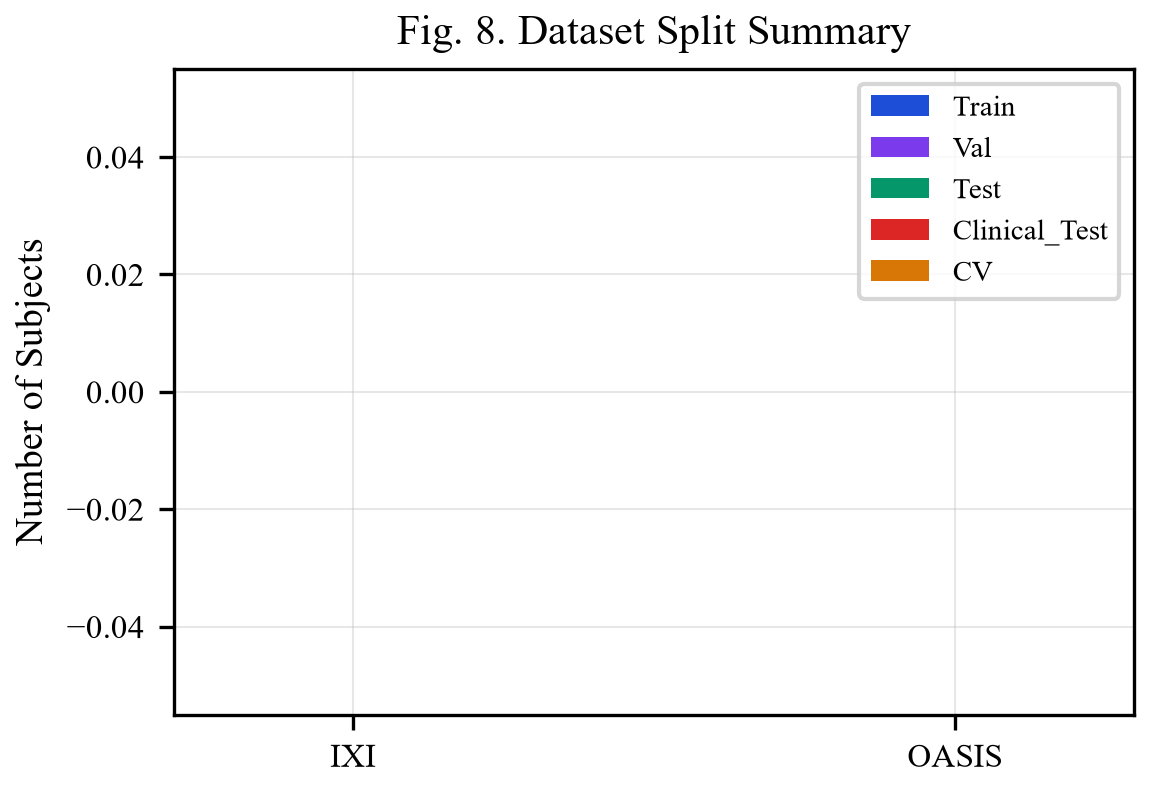
\includegraphics[width=0.62\textwidth]{fig1_cohort.png}
\caption{Partition sizes per cohort stratum ($N=937$: 683 train, 53 validation, 201 test). OASIS-1 test includes 47 healthy and 47 clinical subjects.}
\label{fig:cohort}
\end{figure}

\subsection{Model and inputs}
BrainAgeResNet has a stride-2 3D convolutional stem (16 channels), residual blocks with 32, 64 and 128 channels using Group Normalization~\cite{wu2018group}, and adaptive average pooling, giving a 128-d image representation. The head outputs a distribution over 43 two-year age bins; age is decoded as the expectation $\hat{y}=\sum_k c_k p_k$. Training uses a KL loss to Gaussian soft labels ($\sigma=2$~y) plus a Smooth-L1 term; evaluation uses EMA weights with flip test-time augmentation.

The \textbf{image-only model} uses the 128-d representation only. The \textbf{metadata-assisted model} additionally receives sex, a dataset flag and a cohort-stratum code (WashU 0.0, A 0.25, B 0.50, C 0.75), normalised with training-only statistics and projected to 16-d before concatenation (144-d). It is therefore \emph{not} a brain-only model, and the cohort stratum is both a model input and an audit variable.

\subsection{Calibration and GPR post-processing}
\textbf{Deployable inverse calibration.} We regress the trained CNN's predictions on true age over the 683 training subjects, $\hat{y}=\alpha y+\beta$, giving $\alpha=0.9330$ and $\beta=3.8952$. At inference, $\hat{y}_{\text{deployable}}=(\hat{y}-3.8952)/0.9330$, which needs no chronological age and uses no test labels. \emph{Qualification:} these training predictions come from the CNN trained on the same 683 subjects, so they are in-sample rather than genuine out-of-fold predictions; no separately trained CNN folds were used. The in-sample fit may understate the shrinkage seen on unseen data.

\textbf{Retrospective residual adjustment.} $\hat{y}-(ay+b)$, with $a,b$ fitted on test BAG against true test age. It uses chronological age and is an evaluation-only diagnostic, not a deployable prediction.

\textbf{GPR.} The 128-d latent features of the fixed trained CNN are reduced by PCA (50 components) and standardised, with both fitted inside training folds in five-fold cross-validation and refitted on the full training partition for test prediction. A Gaussian process with RBF and white-noise kernels returns predictive standard deviations (test mean 6.37~y, range 5.97--8.26~y). These are not calibrated confidence intervals; empirical coverage was not evaluated. The GPR cross-validation is conditional on the fixed CNN features and is not end-to-end cross-validation of the CNN+GPR pipeline. The blend $0.79\,\hat{y}_{\text{CNN}}+0.21\,\hat{y}_{\text{GPR}}$ uses a prespecified development weight, not one optimised in the five-fold procedure.

\section{Results}
\subsection{Overall performance and subgroup audit}
On the held-out test cohort ($N=201$) the image-only model had MAE 7.579~y (95\% CI [6.82, 8.42], $R^2=0.787$, mean BAG $+0.491$~y) and the metadata-assisted model 6.938~y ([6.18, 7.77], $R^2=0.813$, $+0.441$~y). Table~\ref{tab:fair} gives subgroup results. The male-minus-female MAE gap was $+0.463$~y (image-only) and $+0.920$~y (metadata); the Stratum~A-minus-Stratum~B gap was $+0.594$~y and $+2.478$~y. These gaps are descriptive: the bootstrap intervals overlap, each model was trained once, and sex, age, dataset and stratum are not independently modelled. The results do not show that either model is fair or unbiased.

\begin{table}[t]
\centering
\caption{Subgroup MAE (years) on the test cohort with 1,000-resample bootstrap 95\% CIs. $\Delta$ = metadata minus image-only. Values are rounded to three decimals; IXI and OASIS-1 rows are source datasets, not strata.}
\label{tab:fair}
\setlength{\tabcolsep}{2.5pt}\small
\begin{tabularx}{\textwidth}{l l r c c r}
\toprule
\textbf{Attribute} & \textbf{Group} & \textbf{$N$} & \textbf{Image-only [95\% CI]} & \textbf{Metadata [95\% CI]} & \textbf{$\Delta$} \\
\midrule
Overall & All & 201 & 7.579 [6.82, 8.42] & 6.938 [6.18, 7.77] & $-$0.641 \\
Sex & Female & 110 & 7.369 [6.18, 8.51] & 6.522 [5.42, 7.65] & $-$0.848 \\
 & Male & 91 & 7.832 [6.73, 8.99] & 7.442 [6.27, 8.73] & $-$0.390 \\
Stratum & B & 32 & 7.366 [5.35, 9.43] & 5.800 [4.45, 7.22] & $-$1.566 \\
 & A & 50 & 7.960 [6.33, 9.72] & 8.278 [6.51, 10.21] & $+$0.318 \\
 & C & 25 & 6.798 [4.53, 9.35] & 7.067 [5.39, 8.91] & $+$0.269 \\
 & WashU & 94 & 7.656 [6.57, 8.77] & 6.579 [5.36, 7.88] & $-$1.077 \\
Dataset & IXI & 107 & 7.511 [6.36, 8.70] & 7.254 [6.18, 8.32] & $-$0.257 \\
 & OASIS-1 & 94 & 7.656 [6.55, 8.78] & 6.579 [5.45, 7.91] & $-$1.077 \\
\midrule
\multicolumn{2}{l}{Male $-$ Female gap} & & $+$0.463 & $+$0.920 & \\
\multicolumn{2}{l}{Stratum A $-$ B gap} & & $+$0.594 & $+$2.478 & \\
\bottomrule
\end{tabularx}
\end{table}

\begin{figure}[t]
\centering
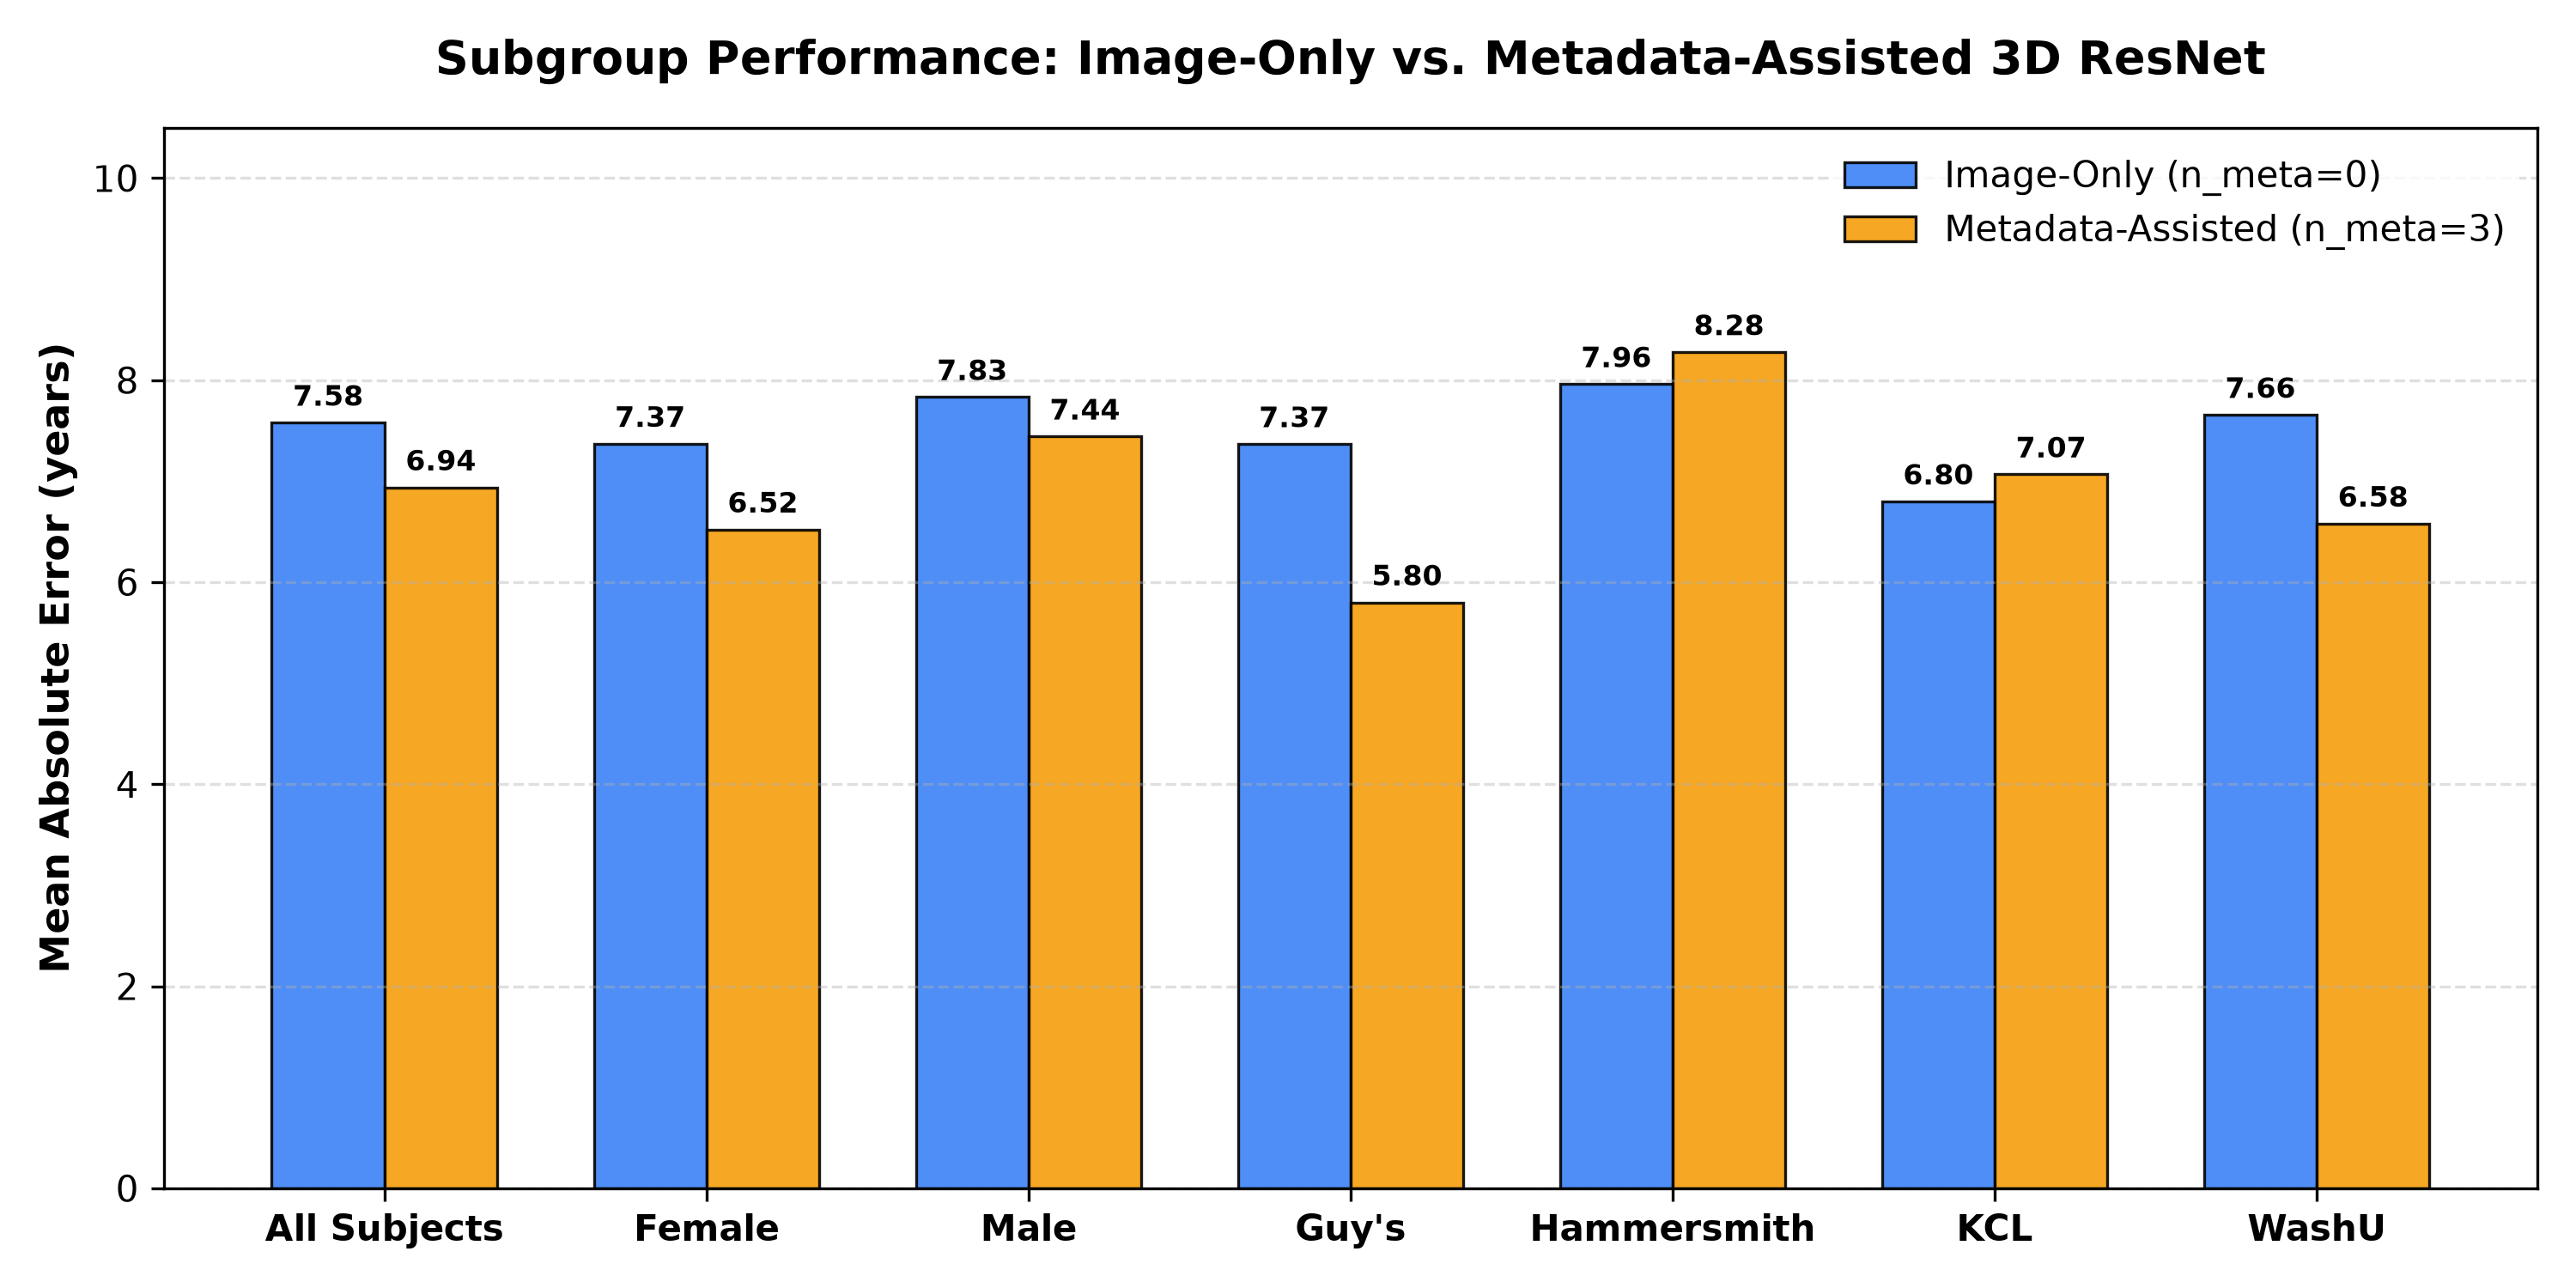
\includegraphics[width=0.66\textwidth]{fig4_subgroups.png}
\caption{Subgroup MAE for the image-only and metadata-assisted models (test cohort, $N=201$; values as in Table~\ref{tab:fair}).}
\label{fig:sub}
\end{figure}

\begin{figure}[t]
\centering
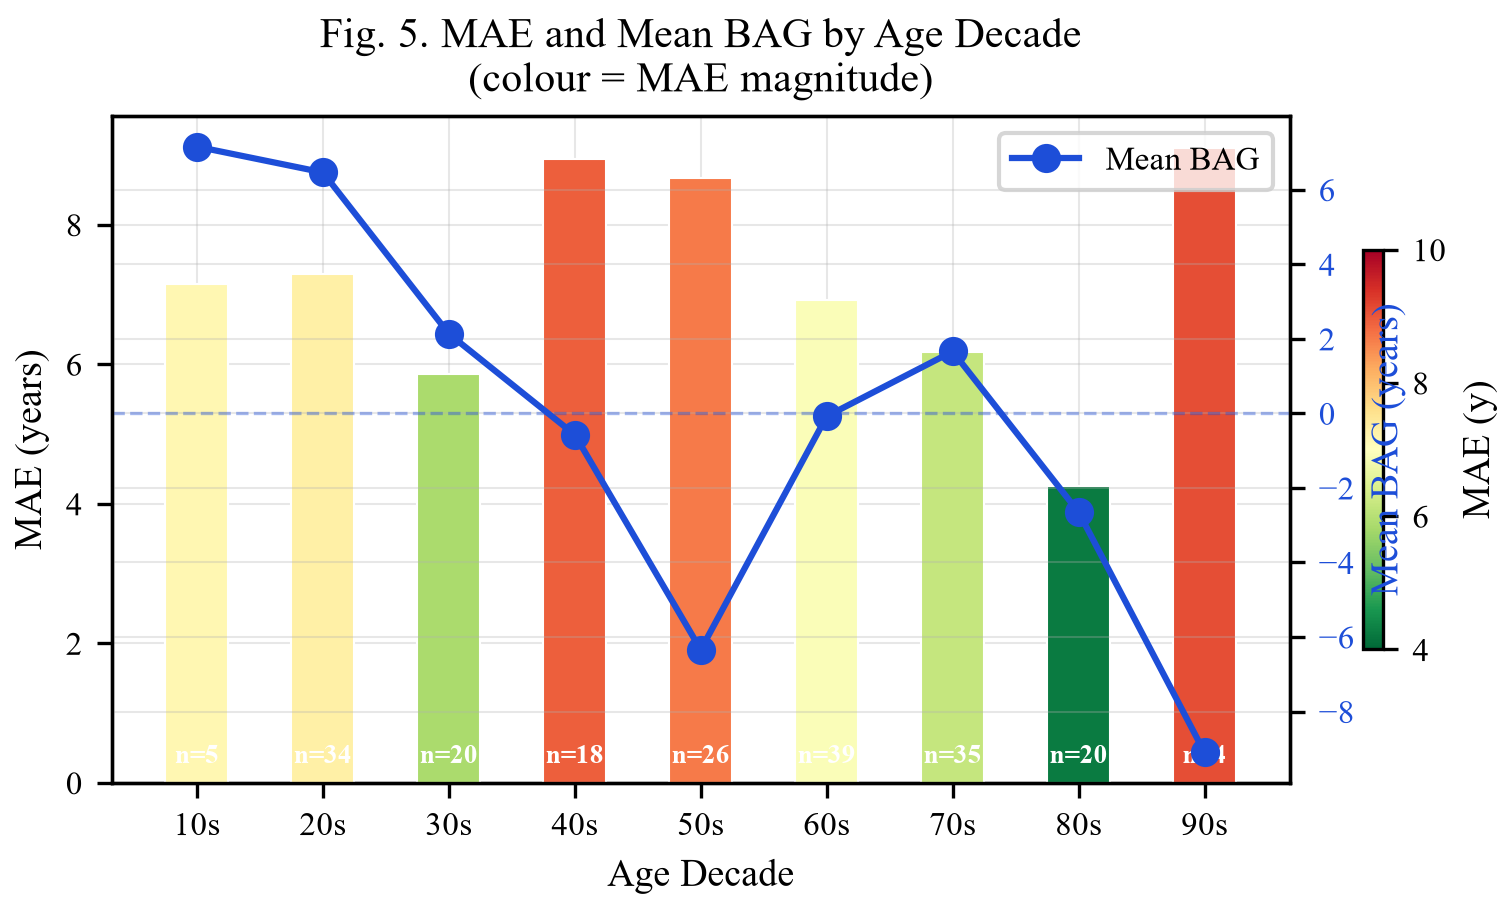
\includegraphics[width=0.66\textwidth]{fig5_decades.png}
\caption{Mean BAG by chronological-age decade (metadata-assisted model), showing regression toward the mean. Decades with $n<10$ (grey) are unreliable.}
\label{fig:dec}
\end{figure}

\begin{figure}[t]
\centering
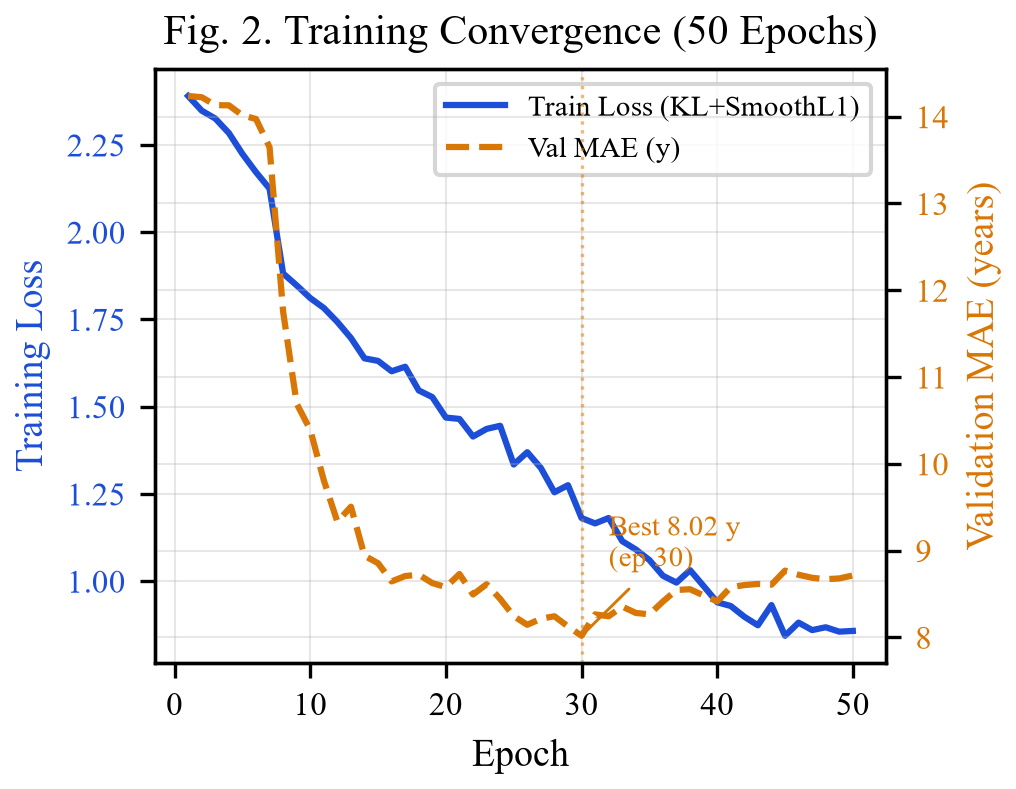
\includegraphics[width=0.62\textwidth]{fig2_training.png}
\caption{Training loss and validation MAE of the metadata-assisted model (best checkpoint at epoch 30, validation MAE 8.02~y, $N=53$).}
\label{fig:train}
\end{figure}

\begin{figure}[t]
\centering
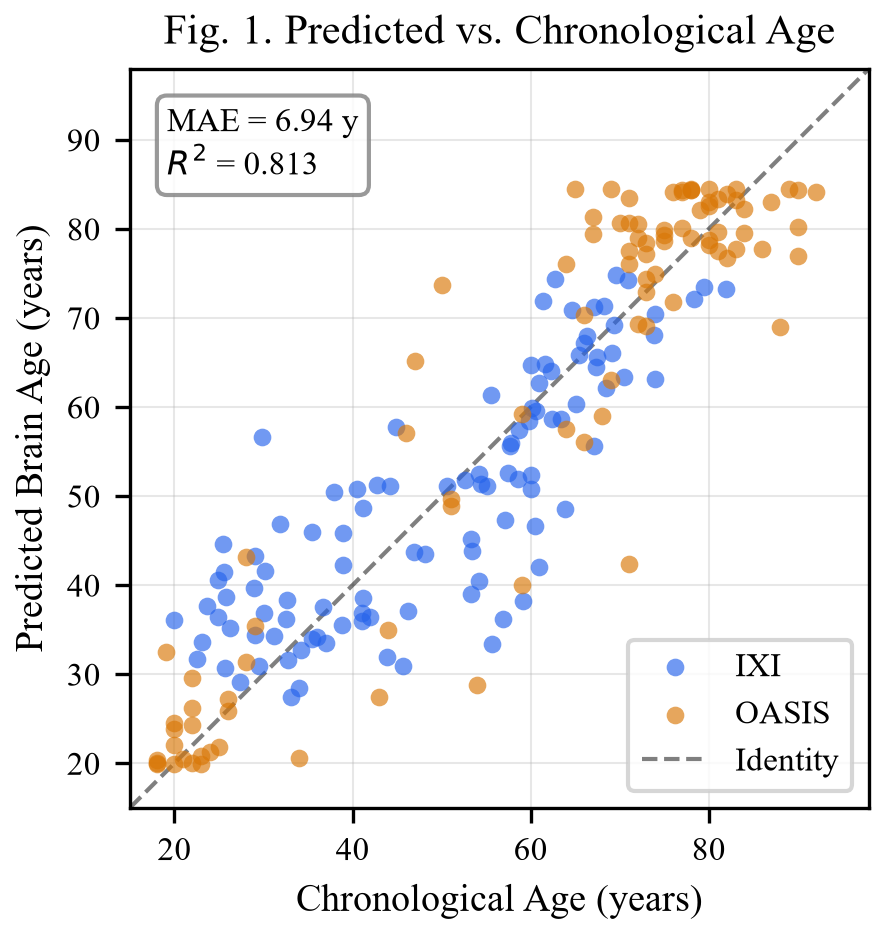
\includegraphics[width=0.55\textwidth]{fig3_scatter.png}
\caption{Predicted versus chronological age on the test cohort ($N=201$, metadata-assisted model).}
\label{fig:scatter}
\end{figure}

\subsection{Model comparison and calibration}
Table~\ref{tab:models} compares stages. Row~1 is an early development baseline evaluated on IXI test scans only ($N=107$); rows 2--7 use the pooled test cohort ($N=201$) and are not directly comparable to row~1. The deployable inverse calibration (MAE 7.218~y) did not improve MAE over the uncalibrated metadata model (6.938~y) but reduced mean bias from $+0.441$ to $+0.229$~y. The retrospective adjustment (6.756~y) uses true age and is a diagnostic only. The blend (6.961~y) was close to the CNN alone.

\begin{table}[t]
\centering
\caption{Model comparison. Row~1: IXI test only ($N=107$). Rows 2--7: pooled test cohort ($N=201$). Row~7 uses chronological age and is not deployable.}
\label{tab:models}
\setlength{\tabcolsep}{3pt}
\begin{tabularx}{\textwidth}{c X r r r r r}
\toprule
\textbf{\#} & \textbf{Model / stage} & \textbf{MAE} & \textbf{$R^2$} & \textbf{Bias} & \textbf{$\pm$5 y} & \textbf{$\pm$10 y} \\
\midrule
1 & Small 3D CNN dev. baseline ($N=107$) & 15.600 & $-$0.190 & --- & 8.4\% & $\approx$30\% \\
2 & Image-only 3D ResNet & 7.579 & 0.787 & $+$0.491 & 40.8\% & 72.6\% \\
3 & Metadata-assisted ResNet (primary) & 6.938 & 0.813 & $+$0.441 & 47.8\% & 75.1\% \\
4 & Standalone GPR & 7.752 & 0.780 & $+$0.211 & 40.3\% & 71.1\% \\
5 & Prespecified CNN+GPR blend & 6.961 & 0.813 & $+$0.393 & 46.8\% & 73.6\% \\
6 & Deployable inverse calibration & 7.218 & 0.798 & $+$0.229 & 44.8\% & 73.6\% \\
7 & Retrospective residual adjustment & 6.756 & 0.827 & $-$0.000 & 45.3\% & 78.1\% \\
\bottomrule
\end{tabularx}
\end{table}

\subsection{Exploratory clinical association (OASIS-1)}
Among the 94 held-out OASIS-1 subjects, mean BAG rose from $-1.29$~y (CDR~0) to $+2.88$~y (CDR~0.5) and $+4.16$~y (CDR~1) (Table~\ref{tab:clin}, Fig.~\ref{fig:clin}). Recomputed from subject-level predictions, healthy controls differed from impaired subjects (Mann--Whitney $U=790$, $p=0.018$), and BAG correlated with MMSE ($r=-0.272$, $p=0.025$, $n=68$). A Kruskal--Wallis test across CDR 0, 0.5 and 1 gave $H=5.97$, $p=0.051$, which is not significant at 0.05; an earlier draft's value ($H=7.82$, $p=0.020$) could not be reproduced and is not used. The CDR~2 group ($N=2$) is too small to interpret. The analysis is exploratory and unadjusted for chronological age; mean age differs strongly by group (CDR~0: 44.8~y, CDR~0.5: 76.4~y, CDR~1: 76.7~y), because healthy test subjects were age-stratified across adulthood.

\begin{table}[t]
\centering
\caption{BAG by CDR in held-out OASIS-1 ($N=94$). SD is the population SD.}
\label{tab:clin}
\begin{tabularx}{\textwidth}{c l r r r r r}
\toprule
\textbf{CDR} & \textbf{Category} & \textbf{$N$} & \textbf{Mean BAG} & \textbf{SD} & \textbf{Median} & \textbf{MAE} \\
\midrule
0.0 & Healthy controls & 47 & $-$1.29 & 10.07 & $-$0.12 & 7.18 \\
0.5 & Very mild impairment & 32 & $+$2.88 & 6.40 & $+$3.64 & 6.02 \\
1.0 & Mild dementia & 13 & $+$4.16 & 6.77 & $+$3.10 & 5.66 \\
2.0 & Moderate dementia & 2 & $-$0.88 & 7.32 & $-$0.88 & 7.32 \\
\bottomrule
\end{tabularx}
\end{table}

\begin{figure}[t]
\centering
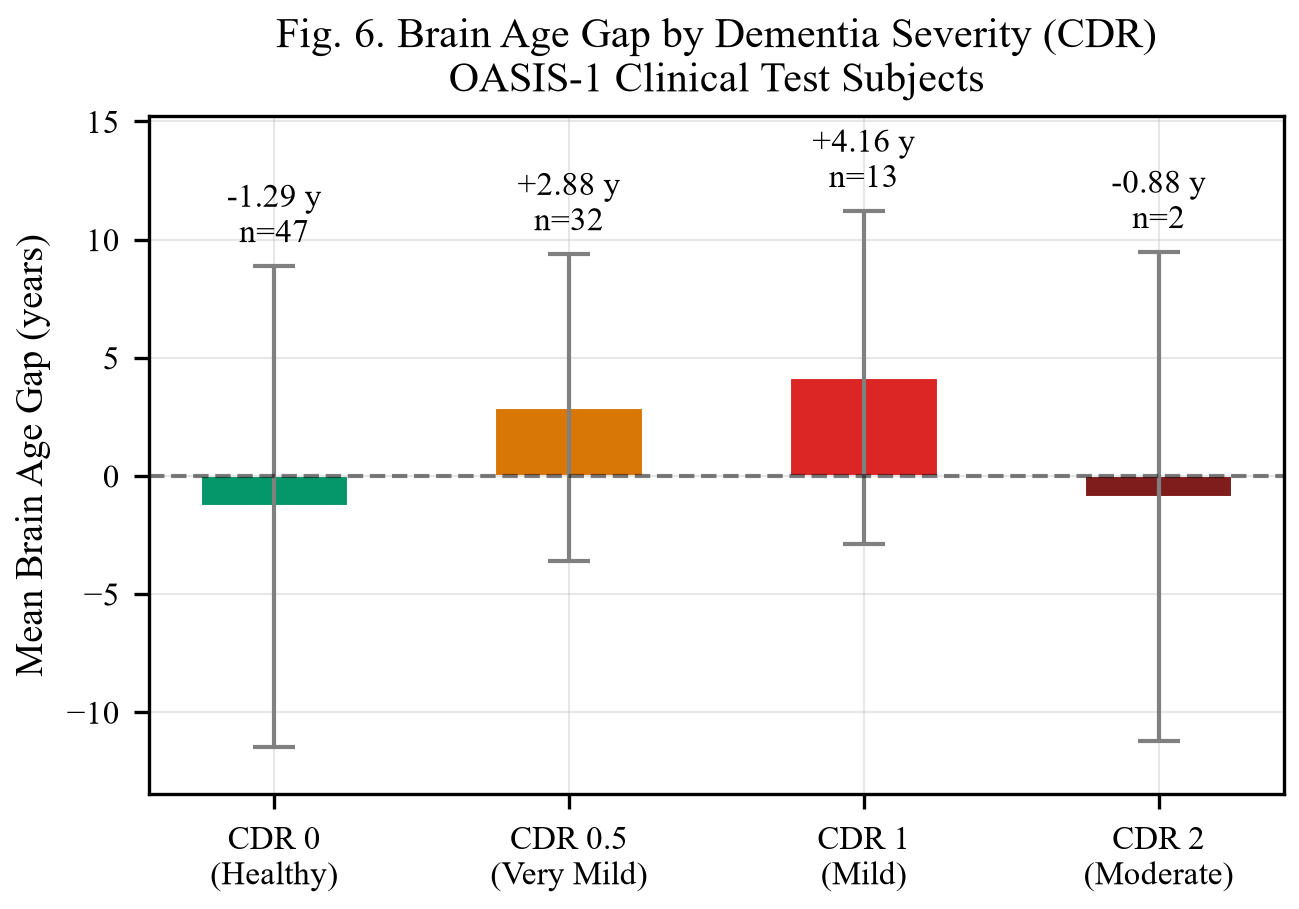
\includegraphics[width=0.48\textwidth]{fig6a_cdr.png}\hfill
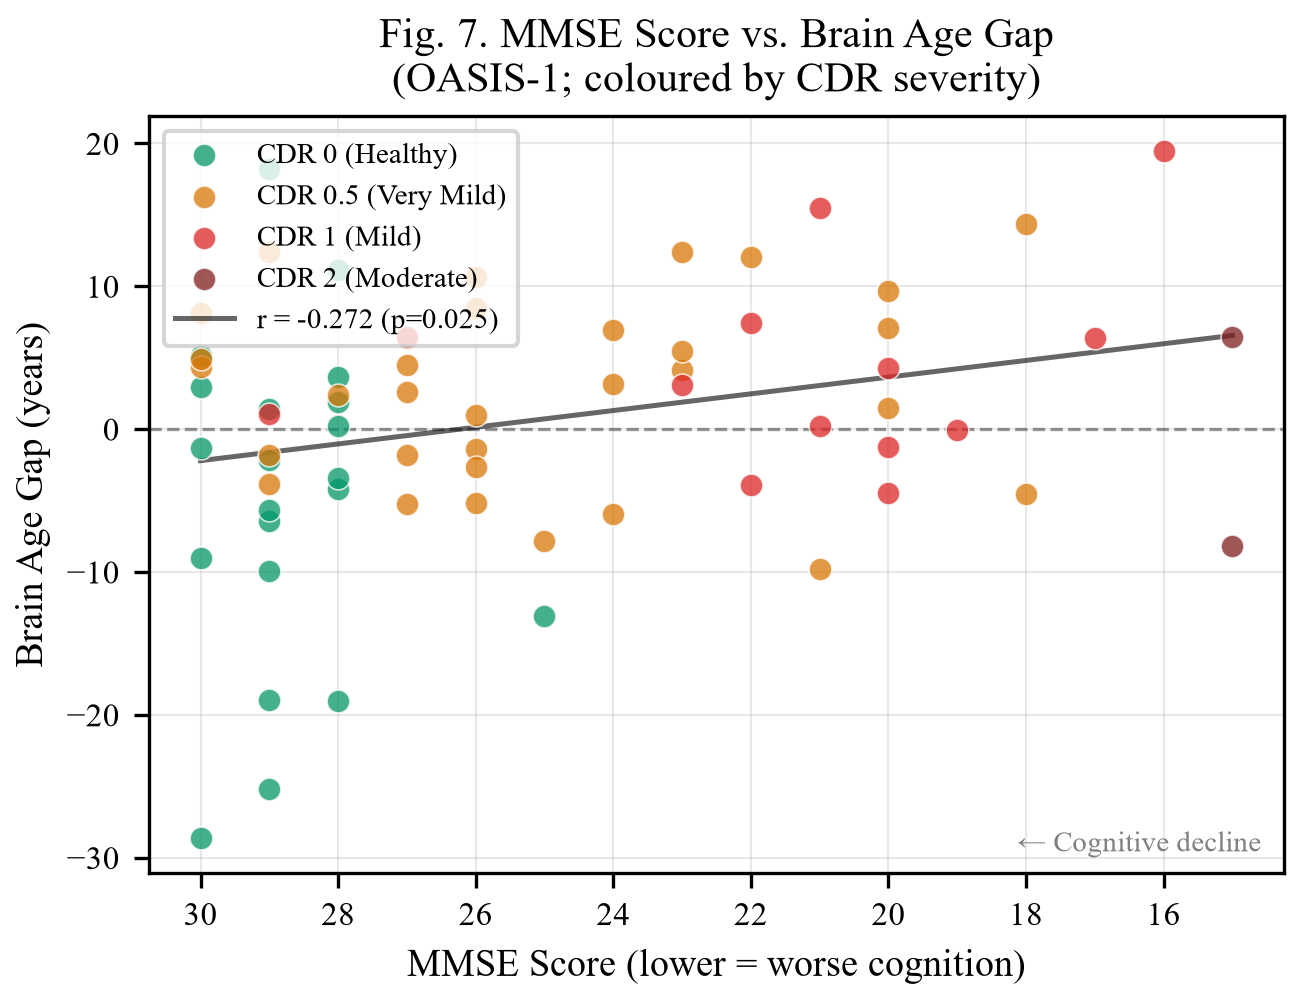
\includegraphics[width=0.48\textwidth]{fig6b_mmse.png}
\caption{(a)~Mean BAG ($\pm$1 SD) by CDR in held-out OASIS-1. (b)~BAG versus MMSE ($n=68$).}
\label{fig:clin}
\end{figure}

\subsection{Proposed reporting checklist}
Table~\ref{tab:check} lists a 10-point checklist and a self-audit (5 met, 3 partly met, 1 open, 1 planned). It is exploratory and needs independent validation.

\begin{table}[t]
\centering
\caption{Proposed reporting checklist and self-audit of this study.}
\label{tab:check}
\setlength{\tabcolsep}{3pt}
\begin{tabularx}{\textwidth}{c p{3.2cm} X l}
\toprule
\textbf{\#} & \textbf{Item} & \textbf{Evidence in this study} & \textbf{Status} \\
\midrule
1 & Subgroup metrics by sex & Table~\ref{tab:fair} (female/male MAE) & Met \\
2 & Cohort strata and dataset provenance & Tables~\ref{tab:cohort}, \ref{tab:fair}; strata documented as non-verified & Met \\
3 & Age-stratified error, low-$N$ flagged & Fig.~\ref{fig:dec} ($n<10$ flagged) & Met \\
4 & Bias-adjustment transparency & Deployable vs.\ retrospective separated; subgroup effect of calibration not studied & Partly met \\
5 & Unseen cohort-stratum generalisation & All strata contribute training data & Open \\
6 & Training-partition demographics & Counts given; full age/sex distributions not tabulated & Partly met \\
7 & Bootstrap confidence intervals & MAE CIs in Table~\ref{tab:fair}; none for all metrics & Partly met \\
8 & Clinical association & CDR and MMSE (exploratory, age-unadjusted) & Met \\
9 & Input-modality declaration & Image-only vs.\ metadata models compared & Met \\
10 & Public code and predictions & Code and crosswalk public; release of per-subject predictions incomplete & Planned \\
\bottomrule
\end{tabularx}
\end{table}

\section{Discussion and Limitations}
In this run, adding metadata lowered overall MAE by 0.641~y, while the observed sex and stratum gaps became larger. We describe these patterns without causal interpretation: intervals overlap, there is one run per model, and the metadata model receives the stratum code directly. Strata are not verified acquisition centres, so no scanner-related explanation is supported.

\textbf{Limitations.} (1)~Single training run per model; no seed variance. (2)~Small validation set ($N=53$, IXI only). (3)~No unseen cohort-stratum evaluation. (4)~Subgroup analyses are descriptive and unadjusted, with small groups (e.g.\ Stratum~C $N=25$; CDR~2 $N=2$). (5)~Dataset composition differs and cohort structure is nested (WashU is OASIS-1 only). (6)~Calibration parameters come from in-sample CNN training predictions. (7)~GPR cross-validation is conditional on fixed CNN features. (8)~The checklist is exploratory. (9)~Clinical associations are not adjusted for chronological age. (10)~IXI crosswalk provenance rests on a documented file-index assumption.

\section{Conclusion}
This preliminary descriptive audit found that metadata input lowered overall MAE (7.579 to 6.938~y) while observed sex and cohort-stratum gaps widened, and that a deployable calibration yielded 7.218~y MAE. Multi-seed runs, an unseen cohort stratum and external validation are needed before any conclusion about subgroup fairness, and we make no claim of clinical utility or of a validated fairness standard.

\subsubsection*{Code availability.} \url{https://github.com/VISHALS566/brain-age-fairness-audit} (revision \texttt{fdbe54e}).

\begin{thebibliography}{10}
\bibitem{beheshti2019bias} Beheshti, I., Nugent, S., Potvin, O., Duchesne, S.: Bias-adjustment in neuroimaging-based brain age frameworks: A robust scheme. NeuroImage: Clinical 24, 102063 (2019)
\bibitem{chen2022transmorph} Chen, J., Frey, E.C., He, Y., Segars, W.P., Li, Y., Du, Y.: TransMorph: Transformer for unsupervised medical image registration. Med. Image Anal. 82, 102615 (2022)
\bibitem{cole2017predicting} Cole, J.H., et al.: Predicting brain age with deep learning from raw imaging data results in a reliable and heritable biomarker. NeuroImage 163, 115--124 (2017)
\bibitem{cole2017trends} Cole, J.H., Franke, K.: Predicting age using neuroimaging: Innovative brain ageing biomarkers. Trends Neurosci. 40(12), 681--690 (2017)
\bibitem{de2020bias} de Lange, A.M.G., Cole, J.H.: Commentary: Correction procedures in brain-age prediction. NeuroImage: Clinical 26, 102229 (2020)
\bibitem{fortin2018harmonization} Fortin, J.P., et al.: Harmonization of cortical thickness measurements across scanners and sites. NeuroImage 167, 104--120 (2018)
\bibitem{franke2010cross} Franke, K., Ziegler, G., Kl{\"o}ppel, S., Gaser, C.: Estimating the age of healthy subjects from T1-weighted MRI scans using kernel methods: Exploring the influence of various parameters. NeuroImage 50(3), 883--892 (2010)
\bibitem{ixi_dataset} IXI Dataset: Information eXtraction from Images. Imperial College London. \url{https://brain-development.org/ixi-dataset/}
\bibitem{marcus2007open} Marcus, D.S., et al.: Open Access Series of Imaging Studies (OASIS): Cross-sectional MRI data in young, middle aged, nondemented, and demented older adults. J. Cogn. Neurosci. 19(9), 1498--1507 (2007)
\bibitem{mehrabi2021survey} Mehrabi, N., Morstatter, F., Saxena, N., Lerman, K., Galstyan, A.: A survey on bias and fairness in machine learning. ACM Comput. Surv. 54(6), 1--35 (2021)
\bibitem{peng2021accurate} Peng, H., et al.: Accurate brain age prediction with lightweight deep neural networks. Med. Image Anal. 68, 101871 (2021)
\bibitem{seyyed2020underdiagnosis} Seyyed-Kalantari, L., et al.: Underdiagnosis bias of artificial intelligence algorithms applied to chest radiographs in under-served patient populations. Nat. Med. 27(12), 2176--2182 (2021)
\bibitem{wu2018group} Wu, Y., He, K.: Group normalization. In: ECCV 2018, pp. 3--19 (2018)
\end{thebibliography}
\end{document}
